\documentclass[12pt,oneside]{article}
\newcommand{\name}{Jean-Yves Djamen}
\newcommand{\class}{Math 80266A}
\newcommand{\hwnumber}{4}

\usepackage[margin=1in,letterpaper]{geometry}
%geometry changes the margins
%inside straight bracket is a parameter, inside curly bracket is name of package or whatever
%

\usepackage{amssymb,amsthm,amsmath,enumerate,fancyhdr,graphicx,tabularx}
\usepackage{float}
\usepackage{microtype}
\usepackage{tikz}
%Enables Graph Theory
\usepackage{pgfplots}
\usepackage{mdframed}
\usepackage[T1]{fontenc}
%Draws fancy boxes
\usepackage{parskip}
%Paragraph skip
\linespread{1.1} 
%Space in between lines
\usepackage{sectsty}
\sectionfont{\fontsize{12}{15}\selectfont}

\newenvironment{problem}[1]
{\begin{mdframed}
%Frames and crap
        \textbf{\textsc{Problem #1:}}
}
{\end{mdframed}}


\newenvironment{solution}
    {\textbf{\textsc{Solution:}}\\}
    {\newpage}

\pgfplotsset{compat=1.16}
\pagestyle{fancy}
\lhead{\textbf{\name}}
\chead{}
\rhead{\textbf{\class\ Assignment\ \hwnumber}}
\rfoot{\thepage}
\cfoot{}
\renewcommand{\headrulewidth}{0.2pt}

%lhead is the left header
%/textbf is text bold header

\def\l{\ell}
\def\pt{\partial}
\def\fish{\mathcal{I}}
\begin{document}

% \begin{enumerate}[I.]
% \item Solution number 1
% \item Solution Dos
% \item 
% \end{enumerate}

%/includgraphics

%/begin{align*}
%Stuff in here
%If star isn't included then the align command will automatically number your crap
%/end{align*}


\begin{problem}{1}
We are interested in the S\&P500, the stock market index that measures the stock performance of 500 large companies listed on stock exchanges in the United States. Three data files are
supplied:
\begin{itemize}
    \item \texttt{SP500-10d.csv:} daily data for the S\&P500 index from October 21, 2010 to October 20, 2020.
    \item \texttt{SP500-10w.csv:} weekly data for the S\&P500 index from October 18, 2010 to October 19, 2020.
    \item \texttt{SP500-10m.csv:} monthly data for the S\&P500 index from November 1, 2010 to October 1, 2020.
\end{itemize}
We focus on the losses suffered on the S\&P500.  Analyze all three datasets using the appropriate tools from extreme value theory. Provide useful insights and risk estimates to investors in the S\&P500.
Provide an executive summary, as well as a more detailed discussion of results referencing supporting tables and figures
\end{problem}

\begin{solution}
We will run standard extreme value analysis on each of the datasets available. For the daily and weekly data we will focus on using the two step fitting mechanism that utilizes an AR(3)-GJR-GARCH(1,1) model to compute the extremes, then a generalized Pareto distribution to model the innovations. From the daily data, we will be able to produce a ``next day" risk estimate and from the weekly data we will be able to produce a ``next week`` risk estimate.


As far as diagnostics, we will be using the Ferro-Segers method to assess the clustering behavior of the scaled innovations, the Box-Ljung test to assess the independence of these residuals, and (only in the daily data case) back testing to assess the performance of the two step EV method. We do not back test weekly data as we do not have enough points for effective back testing.

From the monthly data we will be able to produce an estimate for the maximum loss over 120. months. Because we have less sample points which can be seen to be approximately stationary (shown later), we directly model these using standard GEV analysis methods.

To investors, only the last analysis would matter as the two others give estimates for risk in the past.


\section*{Daily Data}
First let us take a look at the daily losses through time:
\begin{figure}[H]
\begin{center}
{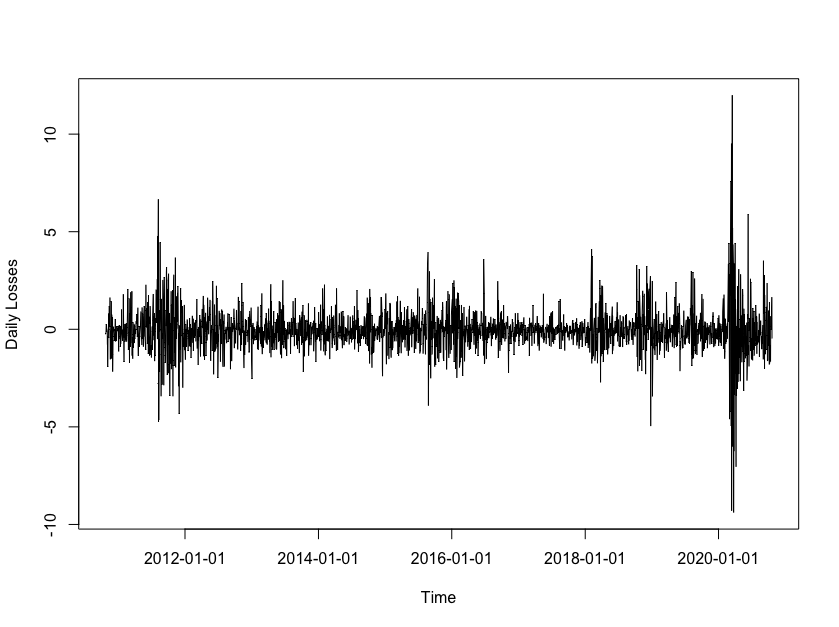
\includegraphics[width=3in]{Assignments/a4/day-data.png}}
\caption{Daily losses of S\&P500 }
\end{center}
\end{figure}
We note sporadic behavior (high volatility) of losses in the beginning of 2020. This is likely due to the effects of the pandemic on the stock market. The effects of COVID-19 on S\&P500 are again reflected in the losses on weekly and monthly data. 

Next, we fit an AR(3)-GJR-GARCH(1,1) model to remove volatility and recover the (hopefully stationary) innovations. Below we compare the ACF plot of observations to the ACF plot of the standardized residuals. As we can note, the standardized residuals have weaker autocorrelation amongst them than the original data. 
\begin{figure}[H]
\begin{center}
{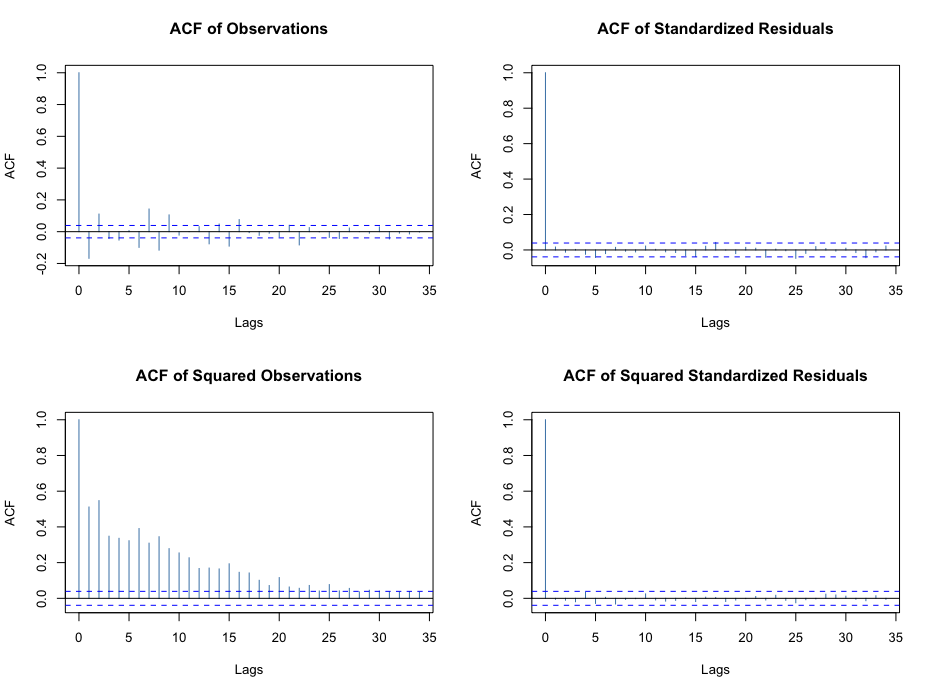
\includegraphics[width=4.5in]{Assignments/a4/day-acfs.png}}
\caption{ACF of standardized residuals and original data}
\end{center}
\end{figure}

Having observed the ACF plots of our residuals we now test the residuals for the having no autocorrelation using the Box-Ljung test. When computing the B-L test on the residuals, we get a $p$ value of $0.4128$ and when performing the test on the squared residuals, we get a $p$ value of $0.7787$. In both cases, we cannot reject the null hypothesis of no autocorrelation. Satisfied that our model removes some of the correlational structure, we evaluate the clustering behaviour of our scaled innovation samples  using Ferro-Segers. Below is the table with our estimates for the extremal index:
\begin{center}
\begin{tabular}{ ||c |c |c|| }\hline
\multicolumn{3}{||c||}{Extremal Index Estimates - Daily Residuals}\\\hline\hline
Threshold & Quantiles& Theta\\\hline
 0.95 & 1.77 & 1 \\ \hline
 0.96 & 1.87 & 1 \\  \hline
 0.97 & 2.07 & 1  \\\hline  
 0.98 & 2.32 & 1 \\ \hline
 0.99 & 2.77 & 1 \\  \hline
\end{tabular}
\end{center}


With the estimate of the extremal index sufficiently close to 1 in all cases, we can proceed to the final step of our modeling process. That is, we fit a generalized Pareto distribution to the exceedences of the scaled innovations using an innovation quantile as the threshold. Below, are the GPD diagnostic graphs from using different quantiles are shown below. From exploratory analysis, we settle with the $u^*=90$ quantile of our scale innovation as the threshold.
\begin{figure}[H]
\begin{center}
{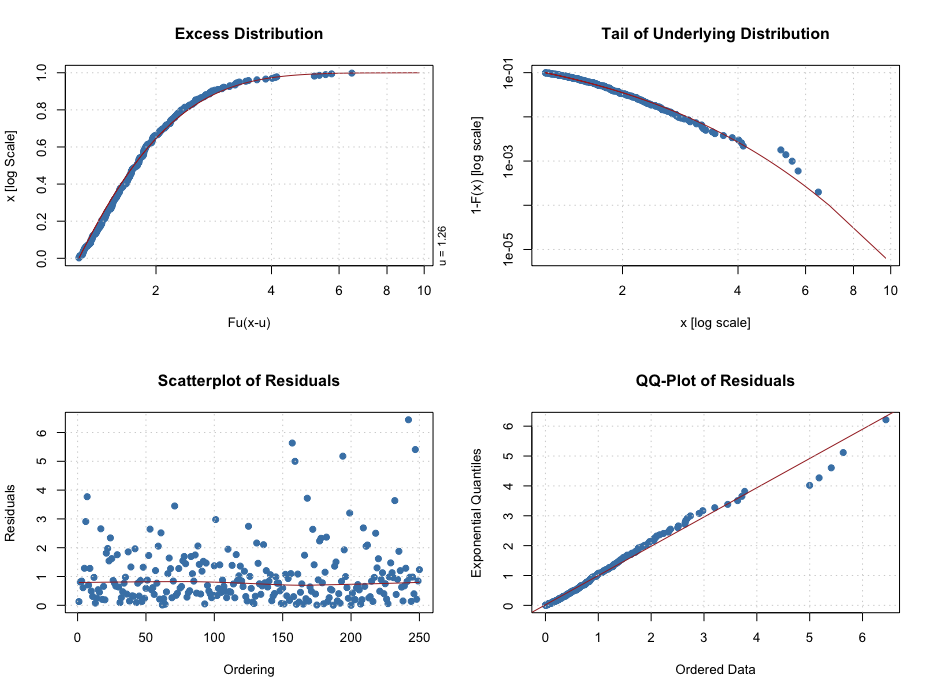
\includegraphics[width=4.5in]{Assignments/a4/90quant-days-gp.png}}
\caption{Threshold is 90$^{th}$ quantile (k=250)}
\end{center}
\end{figure}

\begin{figure}[H]
\begin{center}
{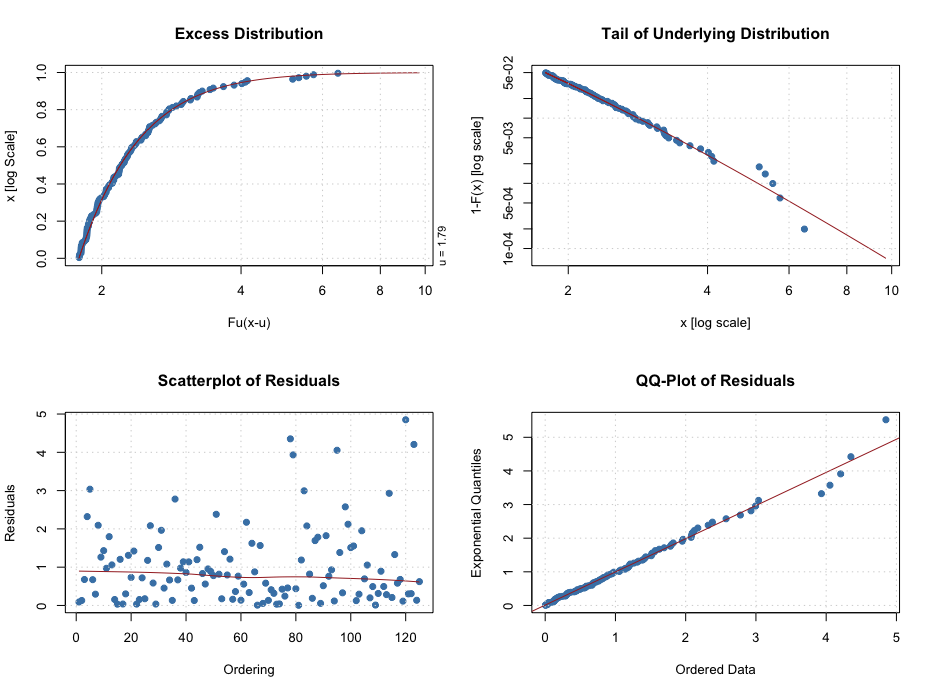
\includegraphics[width=4.5in]{Assignments/a4/95quant-days-gp.png}}
\caption{Threshold is 95$^{th}$ quantile (k=125)}
\end{center}
\end{figure}

\begin{figure}[H]
\begin{center}
{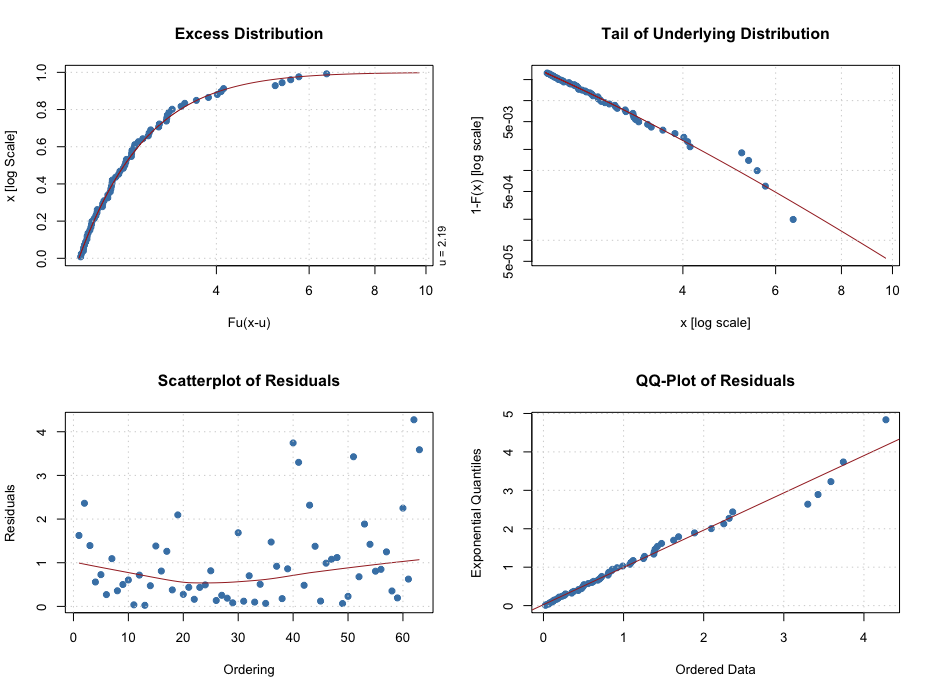
\includegraphics[width=4.5in]{Assignments/a4/97quant-days-gp.png}}
\caption{Threshold is 97.5$^{th}$ quantile (k=63)}
\end{center}
\end{figure}

As you can note, we used our value of $u^*$ because with this threshold, we get the best behaving modeling of the excess distribution, and our qq plot suggest we are less likely to underestimate our upper quantiles. At this step of the analysis, we can now estimate the value at risk and expected shortfall for October 21 2020 to be 3.23 and 4.10 respectively.

\subsubsection*{Backtesting}
Now, we can perform a backtest on our data to justify our use of the two step EV approach. Using the standard window size of 1000 points, we predict a VaR estimate for the next day and compare it to our observed losses. As before, we will estimate, then remove the volatility in order to get estimates for the scaled innovations. These will then be used to fit a GP of excesses over the 90$^{th}$ quantile. Finally, the one step ahead VaR and ES will be estimated and compared to the true values. Below is the graph of losses with shows our the results of our back testing analysis over the last 1516 days of our data.
\begin{figure}[H]
\begin{center}
{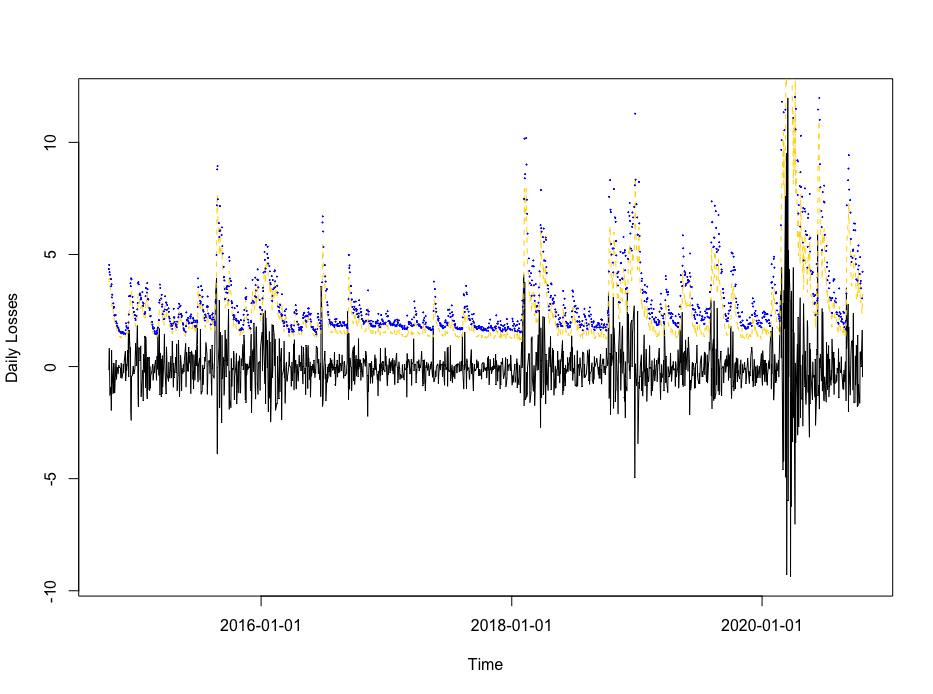
\includegraphics[width=4.5in]{Assignments/a4/backtest-day.png}}
\caption{Backtesting results over the last 1516 days of data. VaR estimates (gold) appear to follow losses. ES also shown in blue.}

{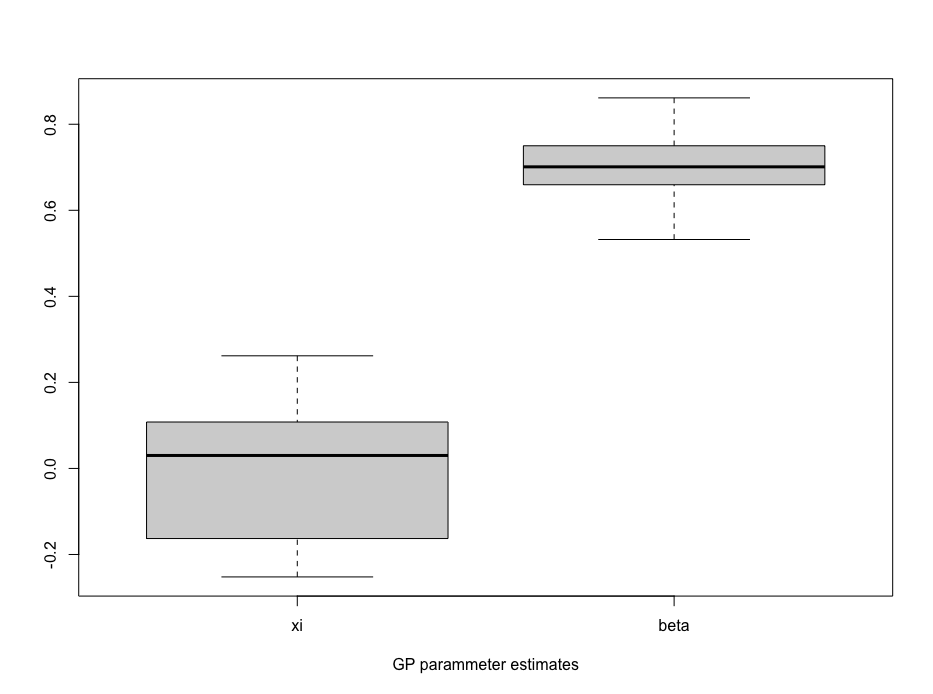
\includegraphics[width=3.5in]{Assignments/a4/back-box.png}}
\caption{GP estimates over backtested data}
\end{center}
\end{figure}

While we might be visually satisfied that our estimate VaR(0.99) estimates seem to contour the losses and the GP estimates for $\xi$ all fall under 0.5 (and thus the QMLE are consistent), we perform a binomial test (alpha=0.05) to determine if the number of wrong VaR estimates is statistically different from what we expected to see. When we do this, we get a p-value of 0.4371 for our 18 violations (expected number of violations is 15.16). This gives an empirical coverage of 0.01187. With these results, we can assume that our analysis was successful and that our approach was sound.

\section*{Weekly Data}
Again, let us begin by taking a look at the data.
\begin{figure}[H]
\begin{center}
{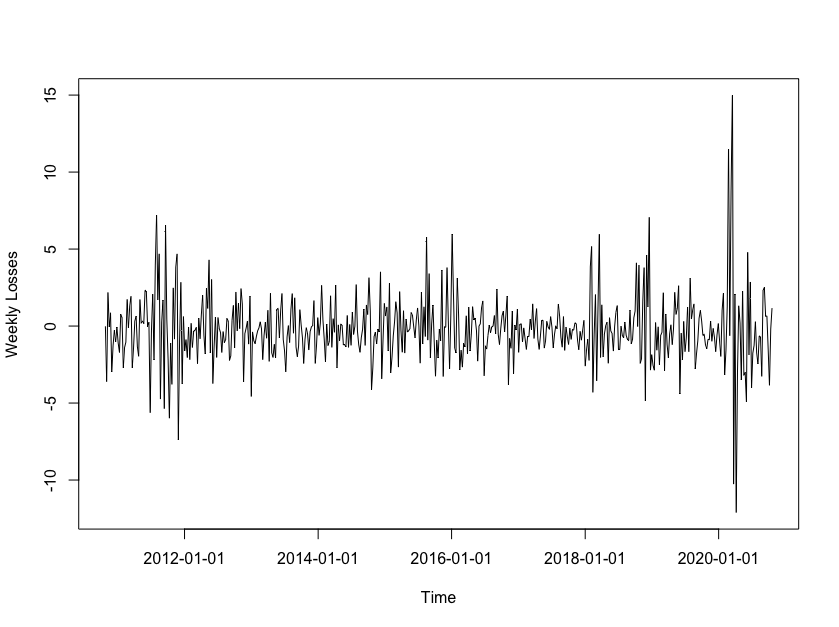
\includegraphics[width=3in]{Assignments/a4/week-data.png}}
\caption{Weekly losses of S\&P500 }
\end{center}
\end{figure}
As before, we fit an AR(3)-GJR-GARCH(1,1) model and observe the diagnostics. 
\begin{figure}[H]
\begin{center}
{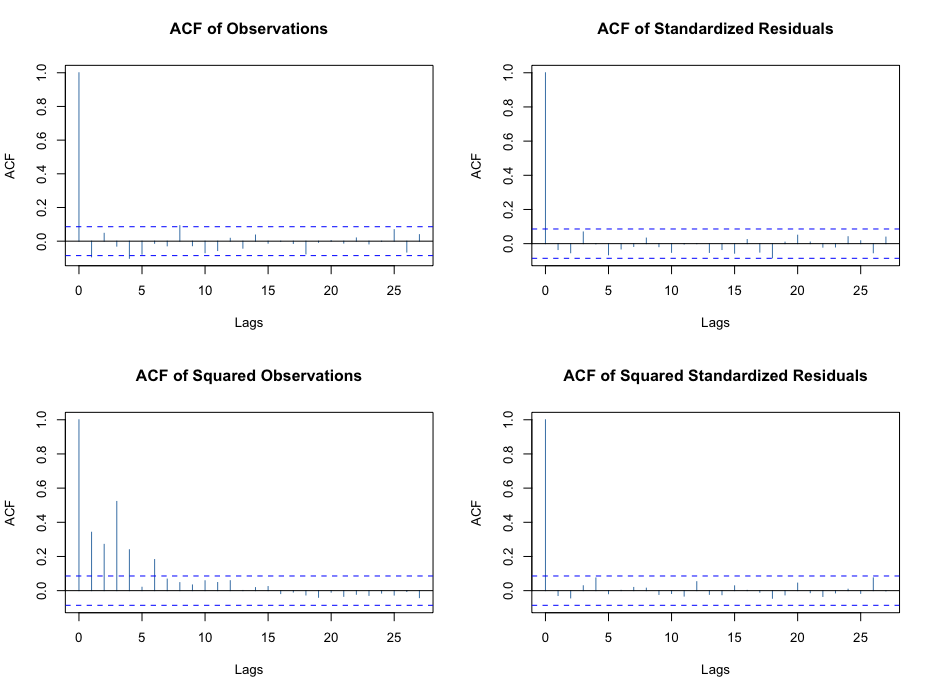
\includegraphics[width=3in]{Assignments/a4/week-acfs.png}}
\caption{ACF or standardized residuals and original weekly data }
\end{center}
\end{figure}
At first glance, week autocorrelation from observations may suggest that we would be well served to assume stationarity of the original data and work from there. However, when performing cluster analysis with on the original data by estimating the extremal index, we notice that the data is far from independent. For this reason, we proceed with the two step EV method.

Using the Box-Ljung test to asses the dependence of standardized residuals and squared standardized residuals, we get p values of 0.4289 and 0.514 respectively. With these, we cannot reject the null hypothesis that the standardized residuals are independent and we proceed to estimating their extremal index (table shown below). Since the estimated extremal indices are close to 1, there is weak evidence of clustering and we can fit our GP to the data.

\begin{center}
\begin{tabular}{ ||c |c |c|| }\hline
\multicolumn{3}{||c||}{Extremal Index Estimates - Weekly Residuals}\\\hline\hline
Threshold & Quantiles& Theta\\\hline
 0.95 & 1.77 & 0.82 \\ \hline
 0.96 & 1.83 & 0.98 \\  \hline
 0.97 & 1.99 & 1  \\\hline  
 0.98 & 2.20 & 1 \\ \hline
 0.99 & 2.73 & 1 \\  \hline
\end{tabular}
\end{center}
Since we have fewer data points, we will need to use a relatively low threshold to ensure that we have enough points to fit a sensible GP to. For this reason, we pick k=55 as this allows us to fit the GPO for exceedences over the 90$^{th}$ quantile.
\begin{figure}[H]
\begin{center}
{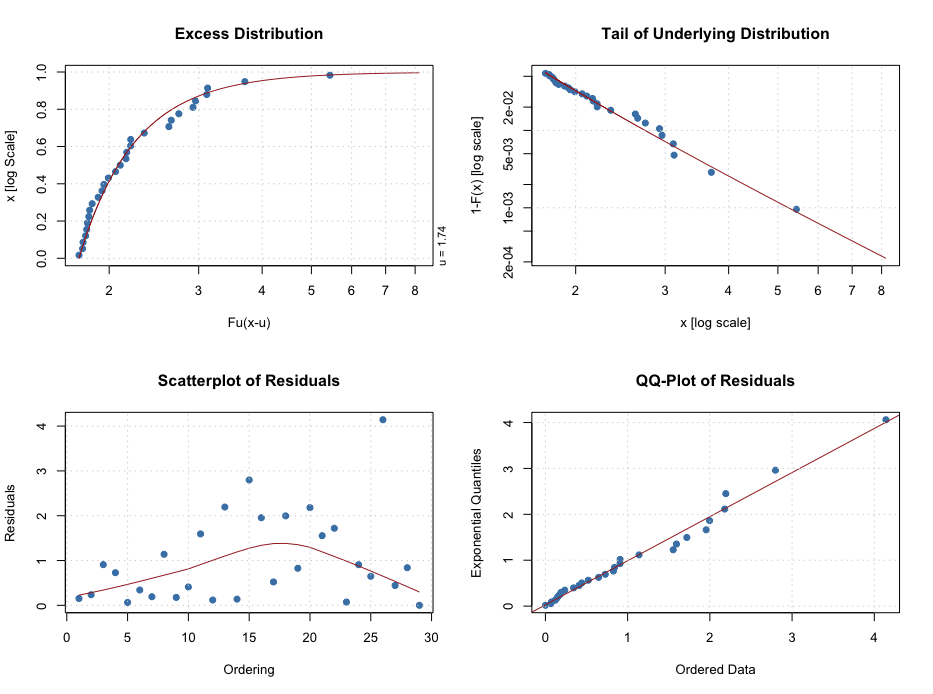
\includegraphics[width=4.5in]{Assignments/a4/55-gp-wk.png}}
\caption{Threshold is 90$^{th}$ quantile (k=55)}
\end{center}
\end{figure}
Using this threshold, we can estimate the VaR for November (up to 19$^{th}$) 2020 to be 4.36 and the ES to be 6.01.

\section*{Monthly Data}
As before, we begin our analysis with a visualisation of the data. Since we do not have many data points to consider, we might want to assess the dependence structure present in our data. This is done using the extremal index estimator and the Box-Ljung test.

\begin{figure}[H]
\begin{center}
{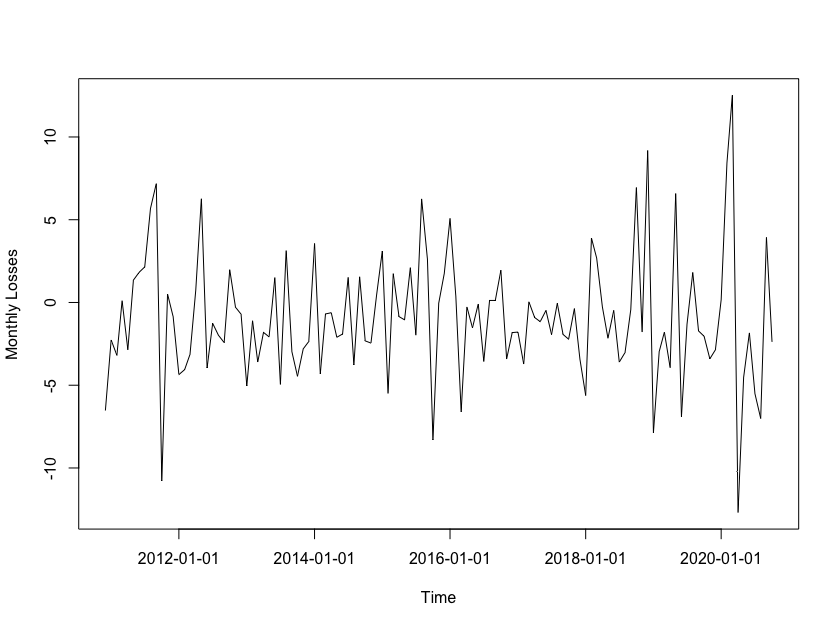
\includegraphics[width=3in]{Assignments/a4/month-data.png}}
\caption{Monthly Losses of S\&P500}
\end{center}
\end{figure}

\begin{figure}[H]
\begin{center}
{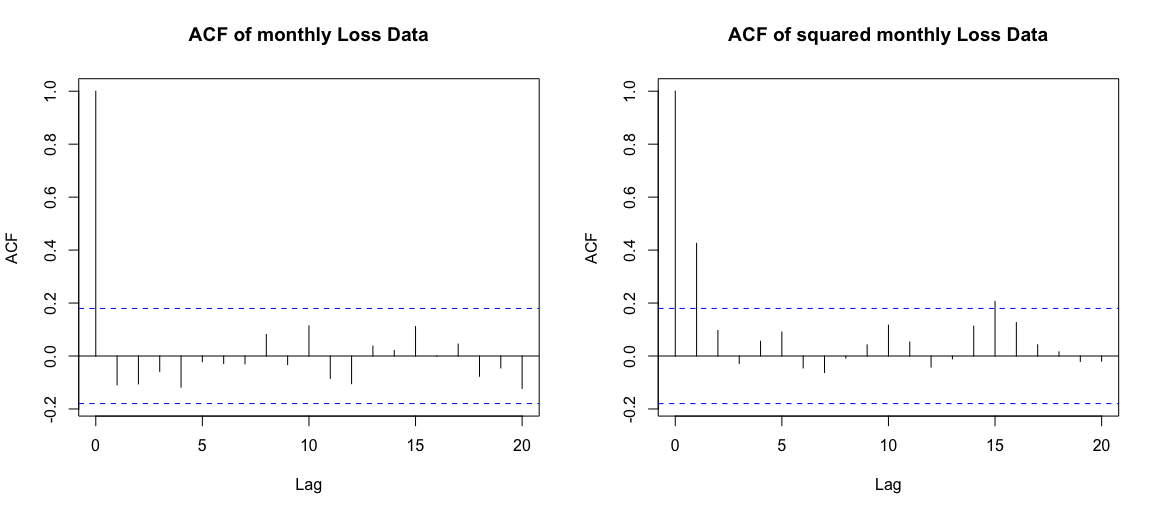
\includegraphics[width=4.5in]{Assignments/a4/mth-acf.png}}
\caption{ACF of monthly data}
\end{center}
\end{figure}
Since the strength of these auto correlations seems low, we proceed with the B-L test and get a p value of 0.228 and cannot reject the null hypothesis that the autocorrelation are not significantly different from 0. From this, we apply the Ferro-Segers extremal index estimator (table below). Using this estimator, we can assume that the high threshold values show low signs of clustering.

\begin{center}
\begin{tabular}{ ||c |c |c|| }\hline
\multicolumn{3}{||c||}{Extremal Index Estimates - Monthly Data}\\\hline\hline
Threshold & Quantiles& Theta\\\hline
 0.95 & 6.26 & 0.534 \\ \hline
 0.96 & 6.58 & 0.674 \\  \hline
 0.97 & 6.94 & 0.875  \\\hline  
 0.98 & 7.18 & 1 \\ \hline
 0.99 & 8.41 & 1 \\  \hline
\end{tabular}
\end{center}

 From these results we will assume the data is stationary and has low volatility that can be estimated (or removed). Therefore, we directly fit a GEV to our data and observe note the performance of our fit.
 \begin{figure}[H]
\begin{center}
{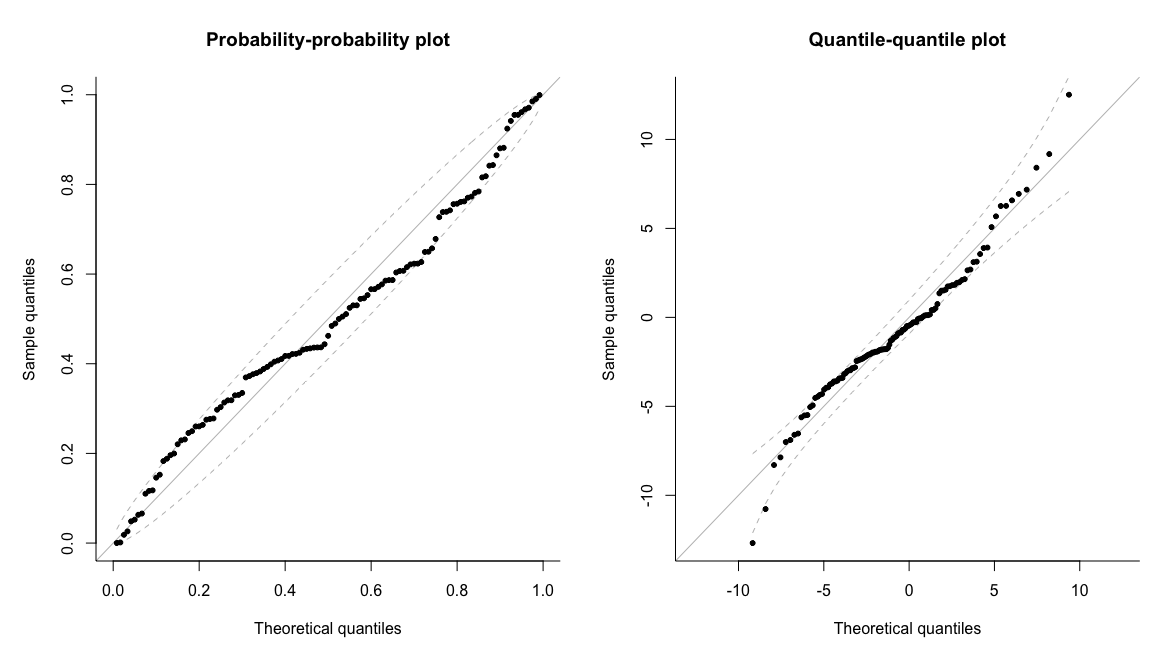
\includegraphics[width=4.5in]{Assignments/a4/month-diag.png}}
\caption{GEV Diagnostic Plot - Monthly Data}
\end{center}
\end{figure}
From the diagnostic plot, we see that while our model may underestimate sample quantiles, these are still covered by the confidence intervals. Therefore, we can proceed with our analysis and make an estimate for the maxima for the return level over 120 months. This value (and the corresponding confidence intervals) will give us the maximum loss we expect to see over the next 10 years. The value is 7.96 and the confidence intervals are   [9.37 11.88].



\end{solution}

\end{document}

